\documentclass[ms]{byuprop}
% Options for this class include the following (* indicates default):
%
%   10pt -- 10 point font size
%   11pt -- 11 point font size
%   12pt (*) -- 12 point font size
%
%   ms -- produce a thesis proposal (off)
%   areaexam -- produce a research area overview (off)
%   phd -- produce a dissertation proposal (off)
%
%   singlespacing -- single-spaced lines
%   doublespacing -- double-spaced lines
%
%   layout -- show layout lines on the pages, helps with overfull boxes (off)
%   grid -- show a half-inch grid on every page, helps with printing (off)


% This command fixes my particular printer, which starts 0.03 inches too low,
% shifting the whole page down by that amount.  This shifts the document
% content up so that it comes out right when printed.
%
% Discovering this sort of behavior is best done by specifying the ``grid''
% option in the class parameters above.  It prints a 1/2 inch grid on every
% page.  You can then use a ruler to determine exactly what the printer is
% doing.
%
% Uncomment to shift content up (accounting for printer problems)
%\setlength{\voffset}{-.03in}

% Here we set things up for invisible hyperlinks in the document.  This makes
% the electronic version clickable without changing the way that the document
% prints.  It's useful, but optional.  Note that if you use latex instead of
% pdflatex, you should change "pdftex" to "ps2pdf".
\usepackage{graphicx}
\usepackage{float}
\usepackage{scrextend}
\usepackage{url}
\usepackage[
    pdftex,
    bookmarks=true,
    breaklinks=true,
    raiselinks=true,
    pdfborder={0 0 0},
    colorlinks=false,
    ]{hyperref}

% Rewrite the itemize, description, and enumerate environments to have more
% reasonable spacing:
\newcommand{\ItemSep}{\itemsep 0pt}
\let\oldenum=\enumerate
\renewcommand{\enumerate}{\oldenum \ItemSep}
\let\olditem=\itemize
\renewcommand{\itemize}{\olditem \ItemSep}
\let\olddesc=\description
\renewcommand{\description}{\olddesc \ItemSep}

% Get a little less fussy about word spacing on a line.  Sometimes produces
% ugly results, so keep your eyes peeled.
\sloppy

% Important settings for the byuprop class. %
%%%%%%%%%%%%%%%%%%%%%%%%%%%%%%%%%%%%%%%%%%%%%

% Because I use these things in more than one place, I created new commands for
% them.  I did not use \providecommand because I absolutely want LaTeX to error
% out if these already exist.
\newcommand{\Title}{Computer Assisted Handwritten Document Transcription Through Subword Spotting}
\newcommand{\Author}{Brian L. Davis}
\newcommand{\SubmissionMonth}{October}
\newcommand{\SubmissionYear}{2015}

% Take these from the commands defined above
\title{\Title}
\author{\Author}
\monthsubmitted{\SubmissionMonth}
\yearsubmitted{\SubmissionYear}

% Committee members
\committeechair{William~A.~Barrett}
\committeemembera{Thomas~W.~Sederberg}
\committeememberb{Daniel~Zappala}

% Department graduate coordinator
\graduatecoordinator{Quinn~Snell}

\documentabstract{%
% The proposal abstract should be 1 to 2 paragraphs.
TODO

Note that there is a blank line between paragraphs, here.
}

%%%%%%%%%%%%%%%%%%%%%%%%%%%%%%%%%%%%%%%%%%%%%

% Set up the internal PDF information so that it becomes part of the document
% metadata.  The pdfinfo command will display this. Be sure to set the document
% type and add your own keywords.
\hypersetup{%
    pdftitle=\Title,%
    pdfauthor=\Author,%
    pdfsubject={Document Type, BYU CS Department: %
                Submitted \SubmissionMonth~\SubmissionYear, Created \today},%
    pdfkeywords={},%
}

% These packages allow the bibliography to be sorted alphabetically and allow references to more than one paper to be sorted and compressed (i.e. instead of [5,2,4,6] you get [2,4-6])
\usepackage[numbers,sort&compress]{natbib}
\usepackage{hypernat}

% Additional packages required for your specific thesis go here. I've left some I use as examples.
%\usepackage{graphicx}
%\usepackage{pdfsync}

\begin{document}

% Produce the preamble
\maketitle

%%%%%%%%%%%%%%%%%%%%%%%%%%%%%%%%%%%%%%%%%%%%%%%%%%%%%%%%%%%%%%%%%%%%%%%%%%%%%%%
\section{Introduction}
At the current rate of FamilySearch's volunteer indexing program, FamilySearch collects documents faster than they can transcribe them. While OCR technology has become accurate enough for tasks in printed document transcription, handwriting recognition has not reached the same level of performance. Accurately transcribing historical documents require a burdensome number of man-hours. This is a problem which faces genealogical record providers, archivists of general historical documents, and applies to a number of tasks related to offline handwriting transcription.

A fully automated, unconstrained handwriting recognition system with an acceptable level of accuracy on historical documents is not possible with the current level of technology. During a recent competition for handwriting recognition on historical documents, the top method had a word error rate above 25\%\cite{icdarComp2015}.  Historical documents have noise, degradation, and other issues which cause accuracies to be lower than other documents. This has left most handwriting transcription work to humans. \iffalse To transcribe (TODO) pages of census documents it took (TODO) man hours.\fi However, there are still ways to leverage recognition techniques to speed up the transcription process, while allowing human oversight and guidance to maintain accuracy. These we will refer to as computer assisted transcription methods (CAT).

The transcription of handwritten historical documents is a service needed by organizations such as genealogical resource providers (FamilySearch, Ancestry, MyHeritage, etc.) and digital archives (the Internet Archive, libraries, etc.). Additionally, the general problem of offline handwriting transcription is highly demanded, evidenced by the numerous businesses offering this service. Those using these services expect human level transcription, but using a CAT method can cut the number of man-hours needed without losing the human oversight.

We have viewed this particularly from the perspective of FamilySearch's volunteer indexing program. Having a better method of transcribing, which is more effective and pleasant to use, would  draw more volunteers to the program. Our transcription paradigm reduces transcription to simple short tasks that could easily be completed by a casual user. It additionally makes it easier to bypass difficult parts of a document, allowing someone else to decipher it. Our paradigm also lends itself to a mobile environment, as it is very adaptable to a small screen and doesn't require typing.

Here, we propose a recognition technique which relies on the key idea that if we can recognize only parts of text, the missing information can be implied by use of a dictionary and language model. This can be compared to the well known game ``Wheel of Fortune'' where players are given a handful of letters, their placement in a phrase/word and a category to aid their guessing. See Fig.~\ref{fig:wheel_of_fortune_example} for an example. In our method, a partial recognition would be achieved by spotting frequently occurring character n-grams in handwritten documents. Character n-grams are useful as they occur with greater frequency than words, and are more distinguishable than individual letters. With this technique, a parallel CAT system could be constructed which allows a computer and multiple humans to work in concert to transcribe a corpus. This system particularly relies on very minimalistic human input (typically selecting things). Additionally, character n-gram spotting can also be used in letter exemplar finding (to aid a human transcriber) or to produce an index for an exemplar free word spotting method.

\begin{figure}[h]
    \centering
    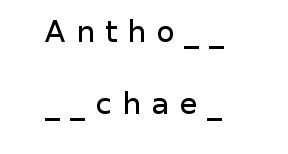
\includegraphics[width=0.25\textwidth]{wheel_of_fortune_example}
    \caption{These are two words with a handful of letters left out. It is not hard to guess the correct words, especially if told these are names. A computer, with access to a dictionary, can be far more effective at this guessing game than a human.}
    \label{fig:wheel_of_fortune_example}
\end{figure}


%%%%%%%%%%%%%%%%%%%%%%%%%%%%%%%%%%%%%%%%%%%%%%%%%%%%%%%%%%%%%%%%%%%%%%%%%%%%%%%
\section{Related Work}

Segmentation is a difficult part of handwriting recognition. While line segmentation techniques are able to accurately extract lines of text and with good success extract words, letter segmentation is an open problem (in the 2009 ICDAR handwriting segmentation contest, multiple entries achieved 99\% line segmentation, the best word segmentation method achieved only 95\% word segmentation accuracy\cite{icdar_segmentation}). Whole word recognition is infeasible for large vocabularies, so we would prefer to recognize individual characters. But to properly segment the letters from a handwritten word (particularly if it is written in a cursive script) is infeasible without having the transcription first. This is Sayre's paradox, where the segmentation and recognition are dependent on one another.\cite{sayres} To solve this, the state-of-the-art approaches have tried to recognize and segment simultaneously.

Hidden Markov models (HMM) were borrowed from speech recognition to achieve this task, and worked reasonably well\cite{Marti2001}. However, HMMs have their own limitations, particularly the Markov assumption and the fact that they are most effective with windows less than the length of a letter, meaning context is often lost.

Recurrent neural networks (RNN) do not share the same limitations as HMMs, and have passed HMMs in performance\cite{Graves2009hmm}. However, they are still lacking the accuracy that is needed for a reliable automatic transcription system; the state-of-the-art results for RNNs (employing long short-term memory blocks) still may have above a 25\% word error rate when transcribing a historical corpus\cite{icdarComp2015}.



Due to the limitations of current handwriting recognition methods we believe that a fully automated handwriting transcription is out of reach. We thus turn our attention to semi-automated recognition approaches, where we are still using a human to transcribe, but also some intelligent recognition technology. A semi-automated solution will outperform a fully automated system in terms of accuracy and is still far more effective than completely manual transcription. Standard CAT approaches use human feedback to correct automatic transcription in an intelligent way, such that it learns something from the corrections. An active learning approach to handwriting transcription is similar to CAT, but is not concerned about achieving human level accuracy, just better accuracy, and thus requires less human involvement~\cite{Serrano2010}. Since we wish to have a system with human comparable accuracy, thus we will focus on CAT approaches.

Toselli, et al\cite{Toselli2007} have explored the realm of CAT using the idea of user-verified prefixes. They use a fairly standard HMM recognition model as the backbone of their approach, and take advantage of the incremental nature of the Viterbi decoding algorithm. The recognition is done for a line of text and the user corrects the first error. The Viterbi is then run again, but this time using the assumption that everything occurring before the correction is correct, and thus reusing the computation up to that point. They have also explored slight variations of the same approach that enable more fluent user input with a touchpad\cite{Toselli2008}, mouse\cite{Toselli2009}, or multimodal\cite{Toselli2010} which speed up the transcription process by allowing more intuitive use interaction. See Fig.~\ref{fig:Toselli_multimodalCAT} Their approach relies on a language model to make corrections on a line when a supervision is made. This means it cannot effectively transcribe documents containing non-sentence writing, such as tables and lists, with this method. Serrano, et al also have pursued a similar approach, where the user corrects the $n$ words in which the recognition model had the least confidence\cite{Serrano2014}.

\begin{figure}[h]
    \centering
    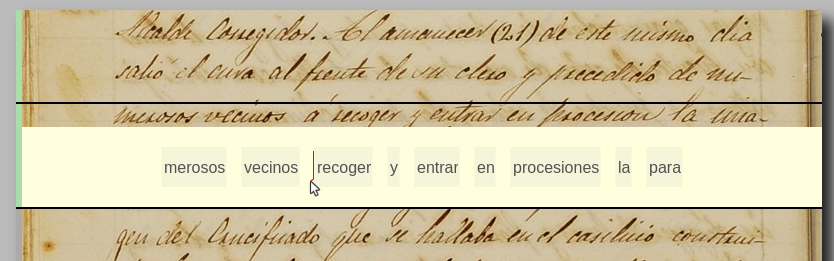
\includegraphics[width=0.95\textwidth]{Toselli_multimodalCAT}
    \caption{A screenshot of a demo of Toselli et al's multimodal CAT system. The red line is drawn by the user to indicate the need to insert a word into the automatically obtained transcription.}
    \label{fig:Toselli_multimodalCAT}
\end{figure}

While it is useful to use an automatic handwriting recognition method as part of a CAT approach to reduce the human burden, we cannot use the same type of recognition used in most CAT systems, where there is a reliance on the predictive capacity of a language model. Some documents are not sentences, and thus cannot be transcribed by these methods. However, many documents are structured such that a pattern can be learned to assist in transcription.

Robert Clawson\cite{Clawson2014}\footnote{You can view a short demo and explanation of his approach at \url{https://www.youtube.com/watch?v=gqdVzEPnBEw}} designed a CAT system for tabular documents, which have a clear pattern. His approach relied on simply finding matches in the document column and assigning them the same user specified label. This provides an accurate CAT system where the user oversees all transcription. The user oversight of matches was accomplished by showing a list of matches to the user (with an adjustable threshold for sensitivity) from which the user removed the false-positive matches. This leveraged the human user's natural ability to discriminate. However, the approach as a whole is limited in that it requires frequent word repetition to be effective. While some tabular documents have this, it is not true for most documents. Additionally, this method had a computation burden where an offline comparison of word similarities was done.

We will show that an alternative to word matching, or word spotting, is character n-gram spotting, as n-grams have more frequent repetition than words do. This will provide the backbone of our CAT system.

Word spotting was first proposed as an alternative to transcribing a corpus. Rather than digitizing the document text image so standard text searches can be run, the document is searched using the images themselves, either with a keyword string or a keyword image (exemplar image). There are two primary approaches to featurize the images when word spotting: holistic features which capture information about a whole image (word) and local or sequential features\cite{Rodrıguez2008}. Holistic features have one description for an entire word image (such as a bag-of-visual-words), where as local features have descriptor for a small portion, or window, of a word image. As local features provide much more detail and are more flexible than holistic features, they have been the most actively pursued in research.

Most of these locally directed feature approaches share the common theme of taking features from vertical slice windows (usually only one or a handful of pixels wide). They compare an exemplar using either dynamic time warping (DTW) or HMMs, relying on a prior line segmentation. The variance between the methods largely lies in the features used. Some use small square windows to allow totally segmentation-free word spotting using a sliding window\cite{Rothacker2013}.

Rodr{\i}guez et al\cite{Rodrıguez2008} proposed a simple histogram gradient feature which they compared against the popular profile and transition based features of Rath and Manmantha\cite{Rath2003}, gradient and transition focused features of Marti and Bunke\cite{Marti2001} and simple histogram features of Bunke et al\cite{Bunke2004}, showing theirs improved performance. They also showed that a HMM worked better than DTW, for their features. However, their method was not an exemplar based approach.

Recently, Aldavert et al\cite{Aldavert2015} and Almazan et al\cite{Almazan2014} have presented superior word spotting methods with rely on heuristic descriptions. Aldavert et al use the well known bag-of-visual-words method, including recent improvements from the Computer Vision community. This is a very simple, yet effective, exemplar spotting approach. Aldavert et al use Fischer vectors, which are similar to bag-of-visual-words, with spatial pyramids in addition to a special pyramids of character histograms to find a new space in training to which both strings and word images can be embedded in. This allows it to preform both string and exemplar queries as well as hybrid queries which yield excellent results.

We are interested in spotting character n-grams (bi- and trigrams) rather than words. While this hasn't explicitly been done, we feel examining the performance of other methods on short words (2 to 3 letters) is instructive. Rothacker et al\cite{Rothacker2013} report $\sim$46\% and $\sim$55\% mean Average Precision (mAP), a drop by $\sim$5\% and $\sim$14\%, for two and three lettered words respectively with their segmentation free HMM based method. Fischer et al\cite{Fischer2012} report $\sim$70\% and $\sim$83\% mAP for two and three lettered words for their line segmentation dependent, character HMM based method. While neither of these numbers are very promising, Almazan et al\cite{Almazan2012} observe that sliding window approaches can frequently find false positives of short words inside other words (e.g.~finding the word ''the'' inside the word ''weather''). As this is precisely what we want to happen in n-gram spotting (we want to find groups of letters in the middle of words), we expect we should have more success spotting character n-grams than other methods in spotting short words. However, part of the poor accuracy in spotting short words is the fact that there is less information with which to discriminate; this is an obstacle we still must overcome.


%%%%%%%%%%%%%%%%%%%%%%%%%%%%%%%%%%%%%%%%%%%%%%%%%%%%%%%%%%%%%%%%%%%%%%%%%%%%%%%
\section{Thesis Statement}

Leveraging straight forward task of character n-gram spotting, we will construct a computer assisted transcription system, focusing on historical documents with limited vocabulary. Our system will use human interaction that is limited to small tasks, which are far easier to complete than typing.
\\
Alternate:
\\
We will construct a computer assisted transcription system which will use character n-gram spotting to create an incomplete transcription of a document. Small tasks completed by users will guide the system to complete the transcription with high accuracy.

%%%%%%%%%%%%%%%%%%%%%%%%%%%%%%%%%%%%%%%%%%%%%%%%%%%%%%%%%%%%%%%%%%%%%%%%%%%%%%%
\section{Project Description}

We will develop a character n-gram spotter, experimenting with modifying existing methods as well as trying ones based on object detection strategies from computer vision. This performance will be empirically measured.

Using the results of the performance of the n-gram spotting, we will evaluate how large of a dictionary our approach is feasible for.

We then will implement a demonstrative transcription tool using the flexibility of n-gram spotting. This will largely be a proof-of-concept work to show how one might use character n-gram spotting. We anticipate its performance to good, but it may be difficult to compare to similar tools as we will be able to direct our tools paradigm differently than others.


\subsection{Spotting}
Our system could be created by using any  horizontal-segmentation free exemplar based word spotting method. However, these are not optimized for the small n-grams we are dealing with.

We require an exemplar based method for a few reasons. One, they tend to be more accurate as the problem is simply matching images with noise. Two, it allows ad hoc identification of new n-grams from the data validated by the user based on a particular author's handwriting. The requirement for at least a horizontal segmentation free method is that it is assumed to be very difficult to segment the letters of a particular word in cursive script.

There are some spotting methods which lend themselves to being able to do both exemplar and sting based queries\cite{Almazan2014}.

\subsection{Preprocessing}
All documents will be have some noise reduction done. They will be deskewed, line segmented, have their text lines deslanted and have the words segmented. Word segmentation will likely have errors, but these can be corrected by users.

\subsection{Dictionary}
Dictionary look-ups with wildcards is a well studied problem. An approach which would be well suited to our needs is n-gram indexing, in which each n-gram has all words which contain it indexed to it. Then a search is simply an intersection of all the indexes for the n-grams in the query.

\subsection{Tool}
The system is designed to leverage to flexible nature of using character n-gram spotting to perform word completion. It is designed to be interactive with multiple asynchronous users, using user feedback to improve its spotting. It is modularized into a handful of program loops and user tasks.

It will begin with a set of n-gram exemplars, or trained n-gram representations obtained offline. Using these we will try to generalize the various forms of handwriting into a handful of examples for each n-gram. These will be used to begin spotting the documents. Depending on the character n-gram spotter's performance, a training step may need to precede the main execution, allowing us to gather context/author specific n-gram exemplars. 

The system is broken in to tasks, some which are completed by the user, some which are completed by a server doing the computation/spotting. By including a task manager which distributes tasks, we can allow for multiple users to be working on the same set of documents simultaneously. See Fig.~\ref{fig:system_diagram} for a brief outline. The tasks to be done by the computation server are as follows:
\\[.5cm]
{\setlength{\parindent}{0cm}
\hspace{2cm} Character n-gram spotting:

\begin{addmargin}[3em]{3em}
Select the most promising n-gram exemplar to spot. Spot that n-gram in the documents. Pass results to user for n-gram verification task.
\\[.5cm]
\end{addmargin}


Dictionary look-up:

\begin{addmargin}[3em]{3em}
When a word has roughly 50\% of its area labelled by n-grams, we create a regular expression representing what we know. This is based on the position of the n-grams in the word, using flexible wildcards to specify possible unrecognized characters and their position. If only a few words are returned by the regular expression (10 or less) we pass this to the user for the transcription selection task.
\\[.5cm]
\end{addmargin}





The tasks presented to the user are as follows:
\\[.5cm]

Character n-gram verification:

\begin{addmargin}[3em]{3em}
The user is shown the n-gram that was spotted and highlighted segments of the images which had positive results. The user discards any false-positives. The assumption is that most should be correct, thus making it easy to pick out those not belonging to the set.
\\[.5cm]
\end{addmargin}

Select correct transcription:

\begin{addmargin}[3em]{3em}
The user is shown the image being transcribed and presented the list of possible transcriptions. The user either selects the correct transcription, or corrects the search by doing one or more of the following:
\begin{itemize}
    \item Splitting the image into two words.
    \item Indicating the image is splicing a word (and which side).
    \item Indicating if either or both of the n-gram labels are wrong.
    \item Manually entering the transcription.
\end{itemize}
If a transcription is selected or entered, a letter alignment is guessed for the word (using the known n-grams as key anchors). The alignment is used to extract author specific n-gram exemplars which are returned to the program.
\\[.5cm]
\end{addmargin}
}

\begin{figure}[h]
    \centering
    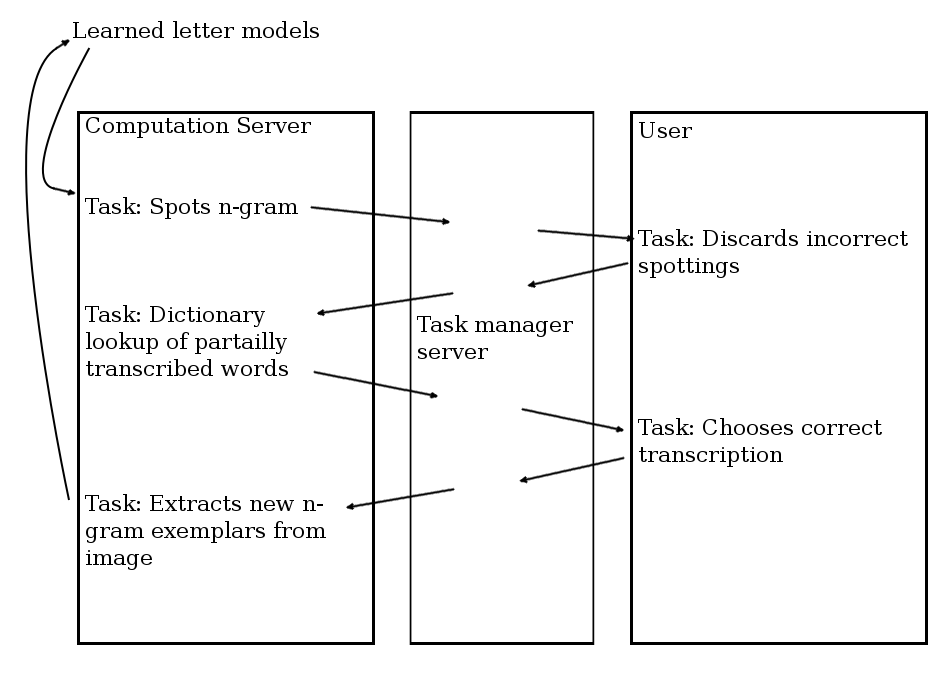
\includegraphics[width=.85\textwidth]{system_diagram_with_arrows}
    \caption{The work-flow of the proposed CAT system. This can support multiple computation servers and multiple users at the same time.}
    \label{fig:system_diagram}
\end{figure}

This method is unique in that the different user's progress will help produce more tasks, making the effort becomes very cooperative. This happens as each completed n-gram verification task will lend labels over a portion of the corpus being transcribed. This allows more possible transcriptions to be found.

This bootstrapping can be done in two ways, using the labeled n-gram as a new exemplar, or using the n-gram as a refining tool to prune images returned by a previous spotting (that haven't been user-reviewed yet). The choice can be decided by evaluating the performance for spotting that particular n-gram: the user's feedback will indicate our false-positive rate, and statistics can estimate our false-negative rate. If our false-positive rate is high, we should prune, if our false-negative rate is high we should use it as another detector.

The testing tool will be developed as a in-browser app, thus making it immediately cross-compatible with all devices with a modern browser. A simple Node.js server will be created to communicate with the clients and the C++ program which will be responsible for performing the actual word spotting.

%%%%%%%%%%%%%%%%%%%%%%%%%%%%%%%%%%%%%%%%%%%%%%%%%%%%%%%%%%%%%%%%%%%%%%%%%%%%%%%
\section{Validation}
The n-gram spotting methods will be empirically tested using well known datasets (George Washington\cite{GW} and IAM\cite{IAM}) as well as a dataset closer to the domain of our expected application of the transcription method.

\subsection{User Study}

The transcription system must be validated with a user study as it's goal is to be a more effective crowdsourcing method for transcription. It is not purely intended to be faster (indeed, it may not be faster than other computer assisted transcription methods), but more modular, allowing for work to be broken up into smaller pieces, and more enjoyable to use. It clearly achieves modularity in design, but we want to see how fast it is and get user feedback to see if it is something people would enjoy using.

Most other computer assisted transcription methods rely on a more fully automated transcription upfront and report performance measures in terms of word error rate or effort reduction, which are measures of how many words the user had to correct. While our users will primarily be doing corrections as well, they will very different types of corrections (taps and swipes instead of typing). Thus it would be difficult to compare these other methods to our proposed method using the previously used metrics.

We propose doing a user study which would involve having a volunteer use the system for some amount of time and then completing a survey about their experience.

%%%%%%%%%%%%%%%%%%%%%%%%%%%%%%%%%%%%%%%%%%%%%%%%%%%%%%%%%%%%%%%%%%%%%%%%%%%%%%%
\section{Thesis Schedule}
\begin{table}[H]
\centering
\begin{tabular}{ll}
Finalization of spotting method          & 1 February 2016 \\
Complete implementation of UI/backend    & 1 April 2016    \\
Complete user tests                      & 15 April 2016   \\
Complete revisions                       & 1 May 2016      \\
Complete additional user tests           & 15 May 2016     \\
Thesis written (all but final revisions) & 7 June 2016     \\
Thesis defended                          & 1 July 2016    
\end{tabular}
\end{table}


%%%%%%%%%%%%%%%%%%%%%%%%%%%%%%%%%%%%%%%%%%%%%%%%%%%%%%%%%%%%%%%%%%%%%%%%%%%%%%%
% Change these to reflect the bibliography style and bibtex database file you want to use
\bibliographystyle{plainnat}
\bibliography{bib}

\end{document}
